\chapter{ROBUSTNESS OF MCF CUT ALGORITHM} \label{ch:robustness}% Must have a blank line after every section label

\section{Introduction} \label{sec:robustness introduction} % Must have a blank line after every section label

\say{Standard form} is the usual and most intuitive form of describing a linear programming problem. It consists of the following three parts:
\begin{itemize}
\item A linear \say{cost} function to be minimized
e.g. $ z(x_{1},x_{2}) = c_1 x_1 + c_2 x_2$
\item Problem constraints of the following form, e.g.
\begin{equation}
\begin{matrix}
  a_{11} x_1 + a_{12} x_2 &\geq b_1 \\
  a_{21} x_1 + a_{22} x_2 &\geq b_2 \\
  a_{31} x_1 + a_{32} x_2 &\geq b_3 \\
\end{matrix}\end{equation}
\item Non-negative variables, e.g.
\begin{equation}\begin{matrix}
 x_1 \geq 0 \\
 x_2 \geq 0
\end{matrix}\end{equation}
\end{itemize}

The problem is usually expressed in matrix form, and then becomes:
\begin{equation}
\min \{ %
\mathbf{c} \transpose
\mathbf{x} \;|\;
 A \mathbf{x} \geq \mathbf{b} \land \mathbf{x} \geq 0 \}
\end{equation}

\subsection{Sensitivity} \label{sec:sensitivity}

Every linear program has a corresponding dual program in the form:

\begin{equation}
\min \{ %
\bm{\lambda} \transpose
\mathbf{b} \;|\;
\bm{\lambda} \transpose A \geq \mathbf{c} \transpose \land \bm{\lambda} \geq 0 \}
\end{equation}

The solutions to the dual program provide \say{shadow prices}, which give a range of values over which the solution is optimal.

Small changes to $\mathbf{b}$ will not change the optimal basis, and there is a linear relationship between the change $\Delta \mathbf{b}$ and the change in the objective $\Delta z$.

\section{Experiments} \label{sec:robustness experiments}

Why you can use multigraph and/or variable capacity.

\subsection{Triangle} \label{sec:triangle}

\subsection{Bridges of K\"onigsberg}

\begin{figure}
\centering
\begin{minipage}{0.45\linewidth}
\centering
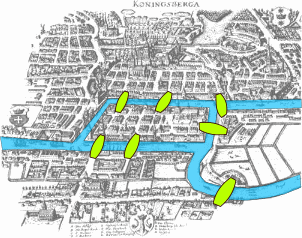
\includegraphics[width=\textwidth]{fig/bridges_map}
\end{minipage}
\begin{minipage}{0.45\linewidth}
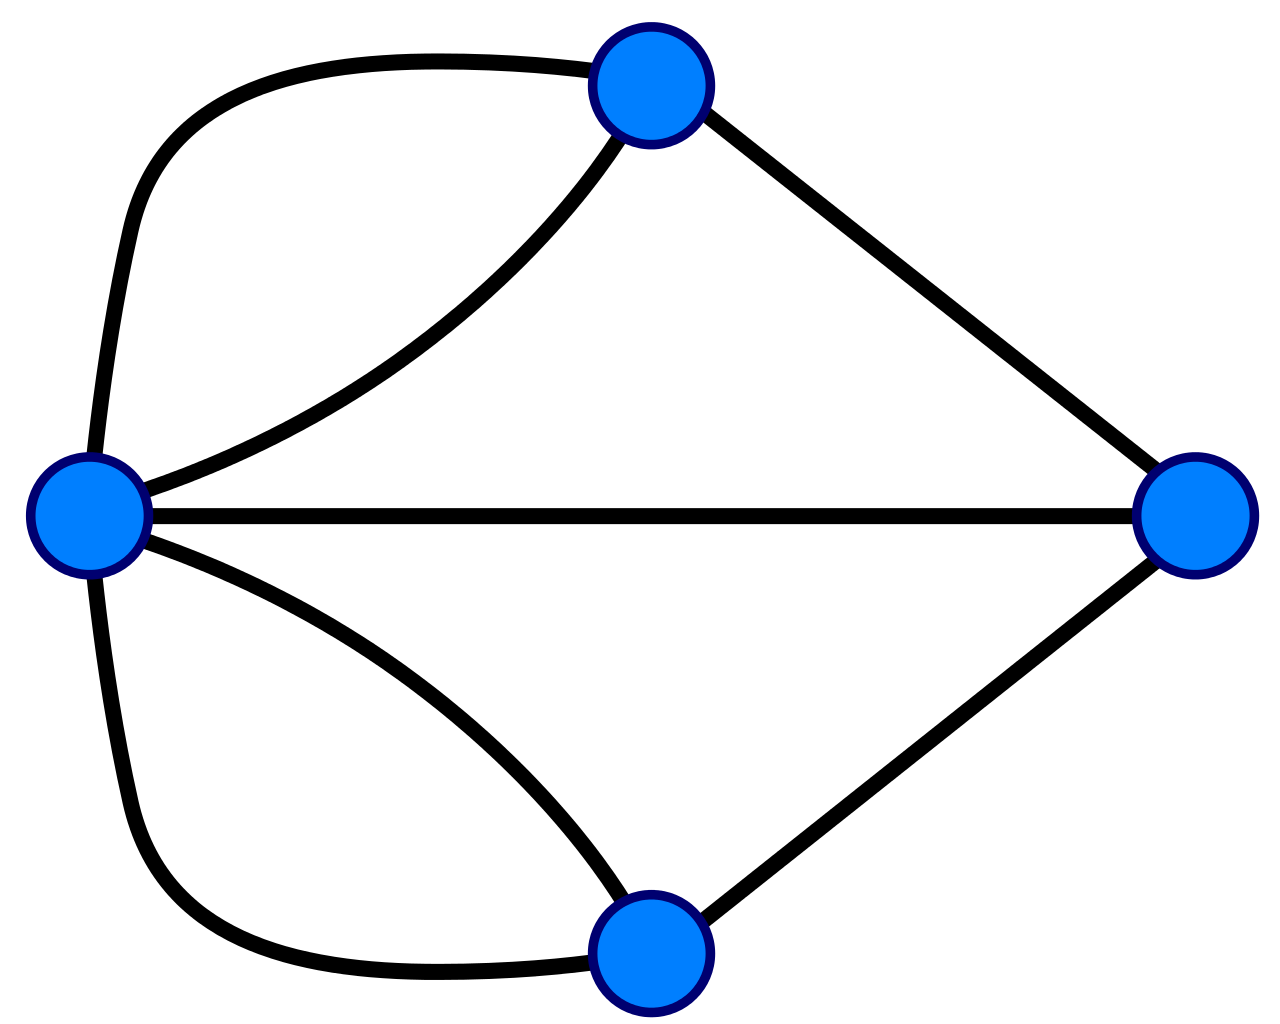
\includegraphics[width=\textwidth]{fig/bridges_graph}
\end{minipage}
\caption{The bridges of K\"onigsberg, as a map and a multigraph}
\label{fig:bridges}
\end{figure}

The bridges of K\"onigsberg spawned the traveling salesman problem (TSP) and what is seen as the first proof in the field of network science~\cite{newman2003structure}. The graph (shown in \autoref{fig:bridges}) is an illustrative example of the 

\subsection{K\textsubscript{3,2}}

\subsection{Florentine families}
